%
%
%

\chapter{Introduction, Review}

%%%%** Section 1
\section{Problem Statement and Learning Objectives}

This week we will review some mathematical basics.

%%%%** Section 2
\section{LODE}
%%%%** Section 2.1
\subsection{Basic definition}

A Linear Ordinary Differential Equation (LODE) is an equation of the form
\[
f(t) = \sum_{i=0}^{N} a_i\frac{d^i}{dt^i}x(t)
\]
The highest derivative, $N$, is referred to as the {\it order} of the LODE.  For example,
\[
f(t) = 0.273\frac{d^3}{dt^3}x(t) + 6.73\frac{d^2}{dt^2}x(t) - 0.001\frac{d}{dt}x(t)
\]
is a third-order LODE.   Often we introduce some shorthand by omitting the time dependence ``$(t)$", and by using the dot notation for time derivatives:
\[
\dot{x} = \frac{d}{dt}x(t)  \qquad \ddot{x} = \frac{d^2}{dt^2}x(t)
\]
So that the example above would be written
\[
f(t) =0.273\frac{d^3}{dt^3}x + 6.73\ddot{x} - 0.001\dot{x}
\]
(you can use three dots for $\frac{d^3}{dt^3}$ if you wish.)


%%%%** Section 2.2
\subsection{Solution of First Order LODE}

A very basic  first order LODE is
\[
\dot{x} + Px = 0
\]

If we guess the solution is
\[
x(t) = e^{pt} \qquad \dot{x}(t) = pe^{pt}
\]
we can easily check it by plugging in to the original LODE:
\[
pe^{pt} +Pe^{pt} = 0 \to pe^{pt} = -Pe^{pt}
\]
giving
\[
p = -P
\]
so the solution is
\[
x(t) = e^{-Pt}
\]

Because of the partial fraction expansion (covered below), this covers a very wide variety of real world LODEs.


%%%%** Section 3
\section{Laplace Transform Review}

We will extensively use Laplace Transforms to manipulate the differential equations of control systems.  As a review, the Laplace transform is
\[
\sL \{f(t)\} = F(s) =  \int_{0}^{\infty} e^{-st}f(t)dt
\]
where $s$ is a complex variable, $s=\sigma + j \omega$.  Technically this is the ``one sided" Laplace Transform because the integral extends only to positive $t$.
The inverse of the Laplace Transform is
\[
f(t) = \sL^{-1}F(s) = \frac{1}{2\pi j} \lim_{T\to\infty} \int_{\sigma - j T}^{\sigma + jT}e^{sT}ds
\]

For this course, we will not need to evaluate these integrals, because all of the LODEs we study will result in just a few terms which have been worked out long ago and are widely available in tables (Table \ref{LaplaceTransformTable}).



%%%%** Table 1
\begin{table}\centering
\renewcommand\arraystretch{2.0}% Vertical Row size, 1.0 is for standard spacing)
\begin{tabular}{|c|c|}
\hline
$ f(t)$ { for} $t \geq 0$ &  $\sL(f)$\\
\hline
$1u(t)$      & $\displaystyle \frac{1}{s}$\\\hline
$e^{at}$ & $\displaystyle \frac{1}{s-a}$\\ \hline
$t^n$    & $\displaystyle \frac{n!}{s^{n+1}}$ ($n = 0,1, \ldots$)\\ \hline
$\sin at$ & $\displaystyle \frac{a}{s^2 + a^2}$\\ \hline
$\cos at$ & $\displaystyle \frac{s}{s^2 + a^2}$\\ \hline
$\dot{f}(t)$ & $s{\cal L}(f)-f(0)$\\ \hline
$\ddot{f}(t)$ & $s^2{\cal L}(f)-sf(0)-\dot{f}(0)$
\\ \hline
\end{tabular}

(Where
$u(t) = \{ 0, t\le 0; 1, t > 0$,
$\dot{f}(t) = \frac{df(t)}{dt}$, $\ddot{f}(t) = \frac{d^2f(t)}{dt^2}$)
\caption{Table of some commonly used Laplace Transform pairs.}\label{LaplaceTransformTable}
\end{table}


When using this table we need to keep in mind a few limitations and assumptions:

\begin{itemize}
  \item We are only considering $t>0$.   One way to do this is to consider functions to be multiplied by the Unit Step function, $u(t)$

\[
  u(t) = \left \{ \begin{array}{ll}  0 & t \le 0 \\ 1 & t > 0 \end{array} \right .
\]

  \item When using the differentiation relationship (last two lines of Table \ref{LaplaceTransformTable}) we must be careful about the initial conditions ($f(0), \dot{f}(0)$).    Most often, we assume that all initial conditions are zero, but it is your responsibility to verify that this assumption applies to a given problem.
\end{itemize}



%%%%** Example 1
\begin{ExampleSmall}
Find the Laplace Transform of the following time functions:  in all cases, assume the function is $0$ for $t<0$ and that initial conditions are zero

\vspace{0.2in}

\[
\sL\{55e^{-1.2t}\}
\]
Consulting the table and using the linearity property of the Laplace Transform integral:

\[
\sL\{55e^{-1.2t}\} = \frac {55} {s+1.2}
\]

\vspace{0.2in}

\[
\sL\{ 3.2\sin(7.6t) \} = \frac {24.32}{s^2 + 57.76}
\]
\vspace{0.2in}


\[
\sL\{ 2.6\ddot{x} - 3.52\dot{x} + 120x \} =
\]
\[
= 2.6X(s)s^2-3.52X(s)s+120X(s)
\]
\[
= X(s) \left(2.6s^2 - 3.52s + 120 \right)
\]
Note that we have assumed that $x(0) = \dot{x}(0) = \ddot{x}(0) = 0$.   Although this seems restrictive, we often consider physical systems starting from rest and this situation is well modeled by such zero initial conditions.
\end{ExampleSmall}


%%%%** Example 2
\begin{ExampleSmall}
Find the inverse Laplace transform of the following functions

\vspace{0.2in}

\[
\sL^{-1}\{\frac{10}{s+3.7}  \}
\]
Consulting the table and using the linearity property of the Laplace Transform integral:


\[
\sL^{-1}\{\frac{10}{s+3.7}  \}  = 10e^{-3.7t}
\]
\vspace{0.2in}


\[
\sL^{-1}\{ \frac{144s}{s^2 + 144} \}  = 144\cos(12t)
\]

\vspace{0.2in}


\[
\sL^{-1}\{ X(s)(s^3 + as^2 + bs+c) \} = \frac{d^3}{dt^3}x + a\ddot{x} + b\dot{x} + cx
\]

Here we have implicitly assumed zero initial conditions.

\end{ExampleSmall}


Let's apply the Laplace Transform to the initial LODE above.  First, we will modify the LODE to include a ``Forcing Function" on the right hand side.  A forcing function is typically a physical input to the system such as an applied voltage or force.

\[
\dot{x} + Px = f(t)
\]
Assuming zero initial conditions and taking the Laplace Transform of both sides (see the second to last line of Table \ref{LaplaceTransformTable}).
\[
sX(s) + PX(s) = F(s)
\]
\[
X(s) (s+P) = F(s)
\]
\[
\frac{X(s)}{F(s)} = \frac {1}  {(s+P)}
\]
Here we have derived a ratio called the ``Transfer Function" between position and the forcing function.  Our solution to the LODE was
\[
x(t) =  e^{pt} =  e^{-Pt}
\]
If we rewrite this using the solution, $p = -P$, then our transfer function becomes
\[
\frac{X(s)}{F(s)} = \frac {1}  {(s-p)}
\]
We call $p$ the ``pole" of this transfer function because the transfer function goes to infinity when $s=p$.



%%%%** Section 4
\section{Partial Fraction Expansion}\label{partialfractionsection}

A very useful property of polynomials is the partial fraction expansion:

\[
\frac{\prod_j (s-z_j)}{\prod_i (s-p_i)}    =  \sum_i  \frac{A_i}{(s-p_i)}
\]

In the form on the left, we have terms called $zeros$ on the top because any time $s=z_i$ the ratio is zero.  We also have terms called $poles$ in the denominator, because any time $s=p_i$, the ratio is infinite.

The partial fraction expansion is very useful for ratios of polynomials in $s$ (such as the left side above) which we will encounter frequently because such a ratio becomes a series of terms which have an easy inverse Laplace Transform
\[
\frac{A_i}{(s-p_i)}   \leftrightarrow  A_ie^{-p_it}
\]
For example,
\[
G(s) = \frac{s+5}{s^3 + 6s^2+ 358s+400}
\]
does not have an obvious inverse Laplace transform.   However if we can factor it to get

\[
G(s) = \frac  {(s+5)}   {(s+2)(s+4)(s+50)}
\]
then we can use the Partial Fraction expansion to  get it into the form
\[
G(s) = \frac{A_1}{(s+2)}+\frac{A_2}{(s+4)}+\frac{A_3}{(s+50)}
\]
then we can immediately write
\[
g(t) = A_1e^{-2t} + A_2e^{-4t} + A_3e^{-50t}
\]





It is not obvious that the partial fraction expansion is always possible but we will derive a class of cases and then perform some examples.

Assume
\[
G(s) = \frac  {(s-z)}   {(s-p_1)(s-p_2)(s-p_3)} =  \frac{A_1}{(s-p_1)}+\frac{A_2}{(s-p_2)}+\frac{A_3}{(s-p_3)}
\]

Now we multiply through by $(s-p_1)$:

\[
G(s) = \frac  {(s-p_1)(s-z)}   {(s-p_1)(s-p_2)(s-p_3)} =  \frac{A_1(s-p_1)}{(s-p_1)}+\frac{A_2(s-p_1)}{(s-p_2)}+\frac{A_3(s-p_1}{(s-p_3)}
\]
Now we do two things:  1) cancel terms where possible,  2) solve for the special case $s=p_1$


1)
\[
\frac  {(s-z)}   {(s-p_2)(s-p_3)} =  \frac{A_1}{1}+\frac{A_2(s-p_1)}{(s-p_2)}+\frac{A_3(s-p_1)}{(s-p_3)}
\]
2)
let $s=p_1$:
\[
\frac  {(s-z)}   {(p_1-p_2)(p_1-p_3)} =  \frac{A_1}{1}+\frac{A_2(p_1-p_1)}{(p_1-p_2)}+\frac{A_3(p_1-p_1)}{(p_1-p_3)}
\]

\[
\frac  {(s+z)}   {(p_1-p_2)(p_1-p_3)} =  {A_1}
\]

We have just solved $A_1$.    If we multiply through by each denominator in turn, we can get all the $A_i$.




%%%%** Example 3
\begin{ExampleSmall}
Expand
\[
G(s) = \frac         {50(s+1)}                      {(s+0.1)(s+14)(s+567)}
\]
by the Partial Fraction Expansion.

\vspace{0.2in}
\[
G(s) = \frac{A_1}{(s+0.1)} + \frac{A_2}{(s+14)} + \frac{A_3}{(s+567)}
\]

\[
A_1 = \left . \frac {(s+0.1)50(s+1)}{(s+0.1)(s+14)(s+567)} \right |_{s=-0.1} =  \frac {50(s+1)}  {(s+14)(s+567)}
\]
\[
= \frac {50(0.9)}{13.9\times566.9} = 0.00571
\]

\[
A_2 = \left . \frac {(s+14)50(s+1)}{(s+0.1)(s+14)(s+567)} \right |_{s=-14} = \frac {50(-13)}{-13.9 \times 553} = 0.0846
\]
\[
A_3 = \left . \frac {(s+567)50(s+1)}{(s+0.1)(s+14)(s+567)} \right |_{s=-567} = \frac {50(-566)}{-566.9 \times -553} = -0.090
\]
\vspace{0.15in}
\[
G(s) = \frac{0.00571}{(s+0.1)} + \frac{0.0846}{(s+14)} + \frac{-0.090}{(s+567)}
\]
\end{ExampleSmall}

%%%%** Example 4
\begin{ExampleSmall}
Use the Partial Fraction Expansion to find the inverse Laplace Transform of
\[
G(s) =  \frac          {27}             {(s+50)(s+3000)}
\]


\[
A_1 = \left . \frac {(s+3000)27}{(s+50)(s+3000)} \right |_{s=-3000} = \frac {27}{-2950} = -0.00915
\]
\[
A_2 = \left . \frac {(s+50)27}{(s+50)(s+3000)} \right |_{s=-50} = \frac {27}{2950} = 0.00915
\]

\[
g(t) = 0.00915(e^{-50t}-e^{-3000t})
\]

\end{ExampleSmall}


In the case that poles are complex conjugates\footnote{Recall that complex poles always come in complex conjugate pairs.}, there are further simplifications possible after the Partial Fraction Expansion.

%%%%** Example 5
\begin{Example}


Find
\[
\sL^{-1}\{G(s) = \frac{(s+5)}{(s+6)(s+2+j)(s+2-j)}\}
\]

\vspace{0.25in}

Using the techniques above we can get:

\[
A_1 = -1/17 = -0.059 \qquad A_2 = 0.029+0.38j \qquad A_3 = 0.029-0.38j
\]
(note that it is not necessary to compute $A_3$ because it will always be the case for complex conjugate poles that $A_3 = A_2^*$.)
\[
G(s)  = \frac {-0.059} {(s+6)}  + \frac {0.029+0.38j} {(s+2+j)}  + \frac {0.029-0.38j} {(s+2-j)}
\]

Applying the inverse transform to each term:

\[
g(t) = -0.059e^{-6t} + (0.029+0.38j)e^{(-2-j)t}+ (0.02-0.38j)e^{(-2+j)t}
\]

First, let's approximate
\[
0.029\pm 0.38j \approx 0.38e^{\pm j \pi/2}
\]
by 1) ignoring the small real part and 2) converting to Magnitude-Angle form.

\[
g(t) = -0.059e^{-6t} + 0.38e^{j\pi/2}e^{(-2-j)t} + 0.38e^{-j\pi/2}e^{(-2+j)t}
\]
\[
g(t) = -0.059e^{-6t} + 0.38e^{-2t} \left ( e^{j(-t+\pi/2)}+e^{-j(-t+\pi/2)} \right )
\]
Now we use Euler's famous equality
\[
e^{j\theta} = \cos(\theta) + j \sin(\theta)
\]
as follows:
\[
g(t) = -0.059e^{-6t} + 0.38e^{-2t} \left (
    \cos(-t+\pi/2) + j\sin(-t+\pi/2)+
    \cos(-t+\pi/2) - j\sin(-t+\pi/2)
    \right )
\]
Since $\cos(\theta) = -\cos(\theta)$, and $\cos(\theta-/pi/2) = \sin(\theta)$

\[
g(t) = -0.059e^{-6t} + 0.38e^{-2t} \left (
    2\cos(t-\pi/2)
    \right )
\]
\[
g(t) = -0.059e^{-6t} + 0.76e^{-2t} \left (
    \cos(t-\pi/2)
    \right )
\]
\[
g(t) = -0.059e^{-6t} + 0.76e^{-2t} \left (  \sin(t)  \right )
\]

\end{Example}



%%%%** Example 6
\begin{ExampleCont}
By throwing a few values of $t$ into the calculator, we can generate a sketch of the second term is shown below:

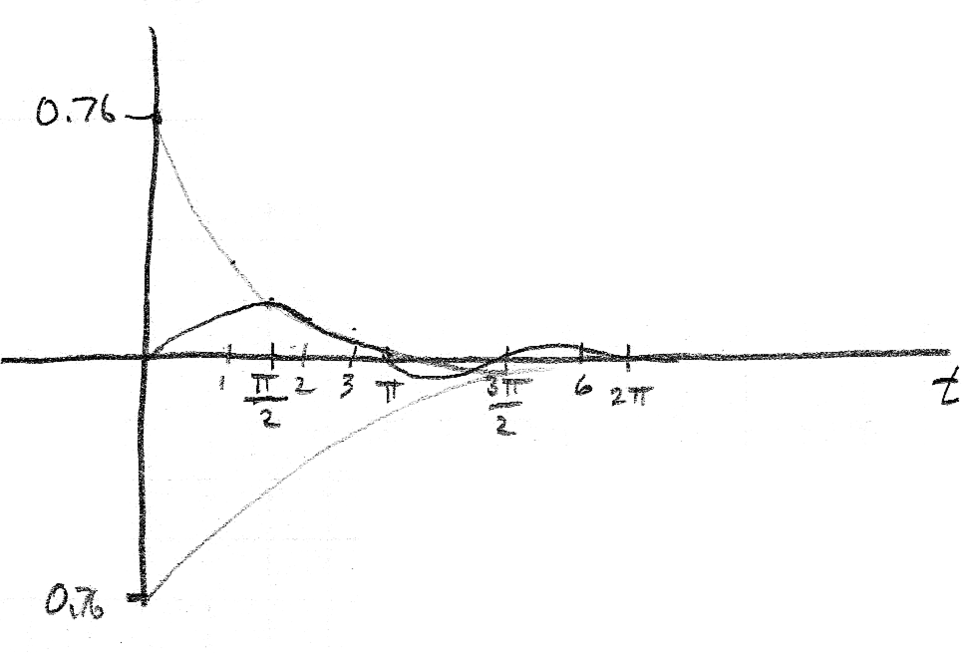
\includegraphics[width=82mm]{figs01/00805a.png}

For a more accurate plot, let's use the computer (including both terms):

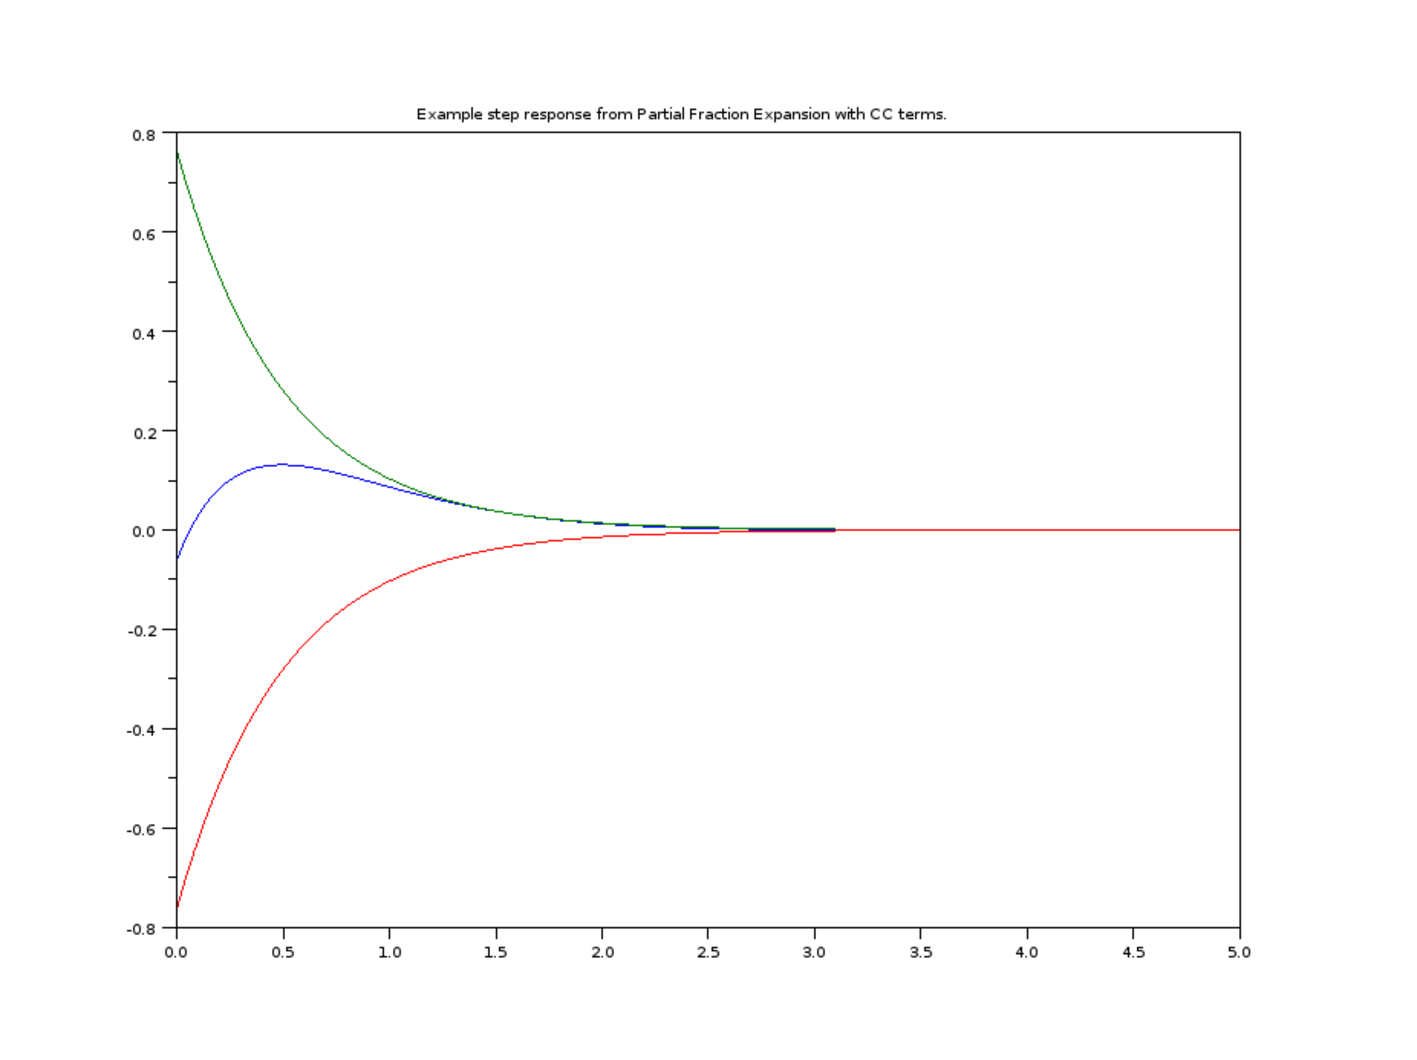
\includegraphics[width=120mm]{figs01/pf_compConja.png}


\end{ExampleCont}


Another situation comes when a pole is repeated (i.e. $\frac{1}{(s+2)^2}$).  In this case the trick we use for the partial fraction expansion no longer works!   But instead we can still solve for $A_i$ by differentiating the partial fraction expansion.

%%%%** Example 7
\begin{ExampleSmall}
Apply the Partial Fraction Expansion to
\[
G(s) = \frac {(s+5)}  {s^2(s+3)}
\]
(noting that there is a repeated root  in the demoninator (repeated pole).

We start by setting up the probelm with two terms for the repeated pole:

\[
G(s) = \frac {A_1}{s^2} +  \frac {A_2}{s} +  \frac {A_3}{(s+3)}
\]
$A_1$:

\[
\left . \frac{s^2(s+5)} {s^2(s+3)}\right |_{s=0}  = \frac {s^2A_1}  {s^2}   + \frac{s^2A_2} {s} + \frac {s^2A_3} {(s+3)}
\]
giving
\[
A_1 = 5/3
\]

$A_3$ is also straightforward, giving $A_3 = 2/9$. But working through $A_2$ we find:

\[
\left . \frac{s(s+5)} {s^2(s+3)}\right |_{s=0}  = \frac {sA_1}  {s^2}   + {A_2}  + \frac {sA_3} {s^2(s+3)}
\]
We now have the problem that we cannot cancel the $s^2$ in the denominator of several terms (which we need to do!).   Instead differentiate the $A_1$ expression with respect to $s$:
\[
\frac{d}{ds}\frac{(s+5)}{(s+2)} = 0 + A_2 + \frac{d}{ds} \frac{s^2}{(s+3)}A_3
\]
\[
\frac{-2}{(s+3)^2} = A_2 + \frac{s(s+6)}{(s+3)^2}A_3
\]
evaluating at $s=0$,
\[
A_2 = -2/9
\]
Note that we have used:
\[
\frac{d}{dx}\frac{(x+a)}{(x+b)} = \frac{1}{(x+b)} - \frac{(x+a)}{(x+b)^2}
\]
and
\[
\frac{d}{dx} \frac{x^2}{(x+a)} = \frac{2x}{(x+a)} - \frac{x^2}{(x+a)^2}
\]

This gets even more unweildy when the repeated pole is non-zero but fortunately we rarely need this technique or can fall back on numerical methods.
\end{ExampleSmall}




%%%%** Section 5
\section{Linearization}

Laplace Transforms can only be used on linear equations.  In most of this course we focus on linear differential equations but often real world applications involve non-linear functions.   All is not lost if we can usefully {\it approximate} our non-linear function with a linear one.  Our approach to linearization is to model the original function with a straight line.


Consider a nonlinear function, $f(x)$.  The linearized version is always constructed about a specific operating point, $x_0$.

\[
\hat{f}(x) = f(x_0) + \frac{d}{dx}f(x_0) (x-x_0)
\]

$\hat{f}(x)$ is a linear function of $x$ which is most accurate in the neighborhood of $x_0$.   It is also the  first two terms of a Taylor series.   It is very helpful to visualize this process graphically by plotting the linearized function on top of the original function.



%%%%** Example 8
\begin{ExampleSmall}

Consider the nonlinear function
\[
f_1(x) = 0.4x^2 -0.1x^3 + 3\sin(x)
\]
and linearize twice, once about $x=-6$, and again about $x=1$.

\vspace{0.2in}

First evaluate $f_1(x)$ for the two linearization points:
\[
f_1(-6) = 36.84 \qquad  f_1(1) = 2.824
\]
Then let's get the derivative:

\[
\dot{f}(x) = 0.8x -0.3x^2 +3\cos(x)
\]
and evaluate it at the two points:

\[
\dot{f}(-6) = -12.72 \qquad \dot{f}(1) = 2.121
\]

Now we get:

\[
\hat{f}_{1a} = 36.84-12.72(x+6) = -39.48-12.72x \qquad \hat{f}_{1b} = 2.824+2.121(x-1) = 0.703+2.121x
\]

Plotting using Scilab:
\begin{center}
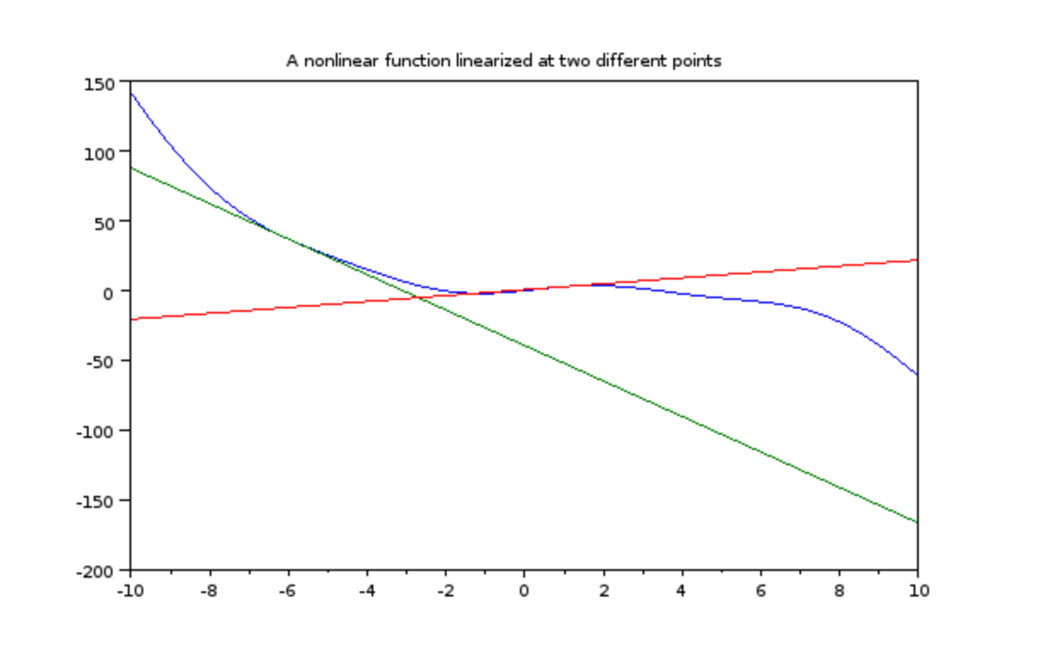
\includegraphics[width=3.5in]{figs01/linearizeattwopointsa.png}
\end{center}

The blue line is $f(x)$, the green line is $\hat{f}_{1a}(x)$ and the red line is $\hat{f}_{1b}(x)$.  The linear approxmations are reasonably accurate in the neighborhood of their operating points, but become very bad as we move away.  The size of the ``neighborhood" for which a degree of accuracy can be obtained depends on the function and the selected operating point.

\end{ExampleSmall}


Some functions are really easy to linearize.

%%%%** Example 9
\begin{ExampleSmall}
Linearize
\[
f_2(x) = 0.723x^3 -4.37x^2 +67x
\]
about the point $x=0$
\vspace{0.2in}

\[
f_2(0) = 0
\]
\[
\dot{f}(x) = 2.169x^2 - 8.74x + 67
\]
\[
\dot{f}_2(0) = 67
\]
\[
\hat{f}_2(x) =  67x
\]
Note that we are simply taking the linear term of $f_2(x)$.   However we only could get away with this because 1) we linearized about $x=0$ and 2) the function was a polynomial.
\end{ExampleSmall}

%%%%** Example 10
\begin{ExampleSmall}
Linearize $f_2(x)$ from the previous example about $x=5.7$
\vspace{0.2in}

\[
f_2(5.7) = 373.81
\]
\[
\dot{f}_2(5.7) = 87.6521
\]
\[
\hat{f}_{2a} = 373.81 + 87.6521(x-5.7)
\]
\[
\hat{f}_{2a} = -125.81 + 87.6521x
\]
This is quite different from $\hat{f}_2(x)$.

\end{ExampleSmall}


When the equation to be linearized is a differential equation, we introduce a slightly strange notion: taking the derivative with respect to a derivative:

%%%%** Example 11
\begin{ExampleSmall}
Linearize the differential equation
\[
f_3(t) =   \ddot{x}(t) - 0.42\dot{x}(t) + 0.01\dot{x}(t)^3 + 16x(t)
\]
about $\dot{x}(t) = 0$.

\vspace{0.2in}
\[
\left . f_3(t) \right |_{\dot{x} = 0} = \ddot{x}(t) + 16x(t)
\]
\[
\frac{d}{d\dot{x}(t)}f_3(t) = 0 - 0.42 + 0.03\dot{x}(t)^2 + 0
\]
for $\dot{x}(t) = 0$,

\[
\left . \frac{d}{d\dot{x}(t)}f_3(t)\right |_{\dot{x} = 0} =   - 0.42
\]

The linearized differential equation is then

\[
\hat{f}_3(t) = \ddot{x}(t) + 16x(t) -0.42\dot{x}(t)
\]

re-writing in traditional LODE form and dropping the $(t)$ for convenience:

\[
\hat{f}_3(t) = \ddot{x} -0.42\dot{x} + 16x
\]




\end{ExampleSmall}

% \section{}
% \section{}
% \section{}
% \section{}
% \section{}



































% \section{Summary of Notation}

